\documentclass[a4paper]{article}
\usepackage[left=2cm, right=2cm, top=0.8in, bottom=1.0in]{geometry}
\usepackage{fontspec}
\usepackage{xeCJK}
\usepackage{indentfirst}
\usepackage{setspace}
\usepackage{paralist}
\usepackage{fancyhdr}
\usepackage[ruled, linesnumbered]{algorithm2e}
\usepackage{setspace}
\usepackage[backref]{hyperref}
\usepackage{amsthm,amsmath,amsfonts,amssymb}
\usepackage{graphicx}
\usepackage{listings,xcolor}
\usepackage{inconsolata}
\usepackage{tikz,forest}
\usepackage{caption, subcaption, amsfonts, dcolumn}
\usepackage{booktabs, multirow, bigstrut, makecell}
\usepackage{lscape}
\definecolor{mygreen}{rgb}{0,0.6,0}  
\definecolor{mygray}{rgb}{0.5,0.5,0.5}  
\definecolor{mymauve}{rgb}{0.58,0,0.82}  
\pagestyle{fancy}
\fancyhf{}
\fancyhead[L]{HTTP-SERVER实验报告 \quad 郭宇祺 \quad 卫思为} %页眉
\fancyfoot[C]{\thepage}
\let\itemize\compactitem
\let\enditemize\endcompactitem
\let\enumerate\compactenum
\let\endenumerate\endcompactenum
\let\description\compactdesc
\let\enddescription\endcompactdesc
\setstretch{1.35} 
\setlength{\parindent}{2em} 
\setmainfont{Times New Roman}
\setCJKmainfont[BoldFont={黑体}, ItalicFont={楷体}]{宋体}
\setCJKsansfont{黑体}
\setCJKmonofont{仿宋}
\renewcommand{\arraystretch}{1.3}
\renewcommand{\figurename}{图}
\renewcommand{\thesubfigure}{(\alph{subfigure})}


\lstset{ %  
  backgroundcolor=\color{white},   % choose the background color; you must add \usepackage{color} or \usepackage{xcolor}  
  basicstyle=\footnotesize\setstretch{1}\setmainfont{Courier New}\bfseries ,        % the size of the fonts that are used for the code  
  breakatwhitespace=true,         % sets if automatic breaks should only happen at whitespace  
  breaklines=true,                 % sets automatic line breaking  
  captionpos=bl,                    % sets the caption-position to bottom  
  commentstyle=\color{mygreen},    % comment style  
  escapeinside={\%*}{*)},          % if you want to add LaTeX within your code  
  extendedchars=true,              % lets you use non-ASCII characters; for 8-bits encodings only, does not work with UTF-8  
  frame=single,                    % adds a frame around the code  
  keepspaces=true,                 % keeps spaces in text, useful for keeping indentation of code (possibly needs columns=flexible)  
  keywordstyle=\color{blue},       % keyword style  
  numbers=left,                    % where to put the line-numbers; possible values are (none, left, right)  
  numbersep=5pt,                   % how far the line-numbers are from the code  
  numberstyle=\tiny\color{mygray}, % the style that is used for the line-numbers  
  rulecolor=\color{black},         % if not set, the frame-color may be changed on line-breaks within not-black text (e.g. comments (green here))  
  showspaces=false,                % show spaces everywhere adding particular underscores; it overrides 'showstringspaces'  
  showstringspaces=false,          % underline spaces within strings only  
  showtabs=false,                  % show tabs within strings adding particular underscores  
  stepnumber=1,                    % the step between two line-numbers. If it's 1, each line will be numbered  
  stringstyle=\color{orange},     % string literal style  
  tabsize=2,                       % sets default tabsize to 2 spaces  
}  
\newtheorem{theorem}{定理}
\begin{document} 
\title{HTTP-SERVER实验报告}
\author{小组成员:郭宇祺 \; 卫思为}
\date{}
\maketitle
\normalsize
\section{实验内容简介}
我们的HTTP服务器实现了三个基本功能:服务器主页获取、文件上传、文件下载。我们在服务器主页获取和文件下载这两个功能上实现了HTTP GET方法,在文件上传这个功能上实现了HTTP POST方法以及分块传输功能。同时我们针对文件上传功能实现了HTTP pipeline。我们还借助openssl库实现了SSL加密,目前我们的服务器只能通过https协议访问,不能通过普通http协议访问。

\section{项目编译与部署}
本项目使用纯C语言开发,使用cmake工具辅助构建。项目编译方法如下:
\begin{lstlisting}[language=bash]
	mkdir build
	cd build
	cmake ..
	make
\end{lstlisting}
上述命令执行完成后会在项目文件夹下生成名为“server”的可执行文件。通过运行“server”即可启动服务器。服务器固定绑定本机5000端口,启动之前请确保本机5000端口空闲,或修改服务器的默认端口。

\section{实现方法}
\subsection{HTTP POST/GET方法}
在本次实验中,由于我们的http-server使用纯C语言编写,因此无法使用高级框架解析请求头,也很难使用高级数据结构存储解析得到的信息。因此,我们使用较为简单的字符串匹配的方法手动实现HTTP请求头的解析。在我们的实现中,我们所实现的HTTP请求头解析功能只会解析与本次实验内容相关的项,对于其他无关项,我们的请求头解析功能不做识别和处理。

HTTP GET方法的实现较为简单。在HTTP请求头中,第一行就包含了本次HTTP请求所访问的URI信息。在http协议中,对于URI,使用符号"?"作为分隔符分隔访问路径与参数,"?"之前的字符串表示所要访问的文件/应用所在路径,之后的字符串表示访问对应文件/应用时所需要的参数。参数以键值对key=value的形式出现,多个参数之间使用"\&"符号进行分隔。基于以上原则,我们编写代码实现了HTTP GET方法的解析功能,相关代码主要集中在lib/server\_handler.c文件中的cut\_params()函数和get\_value()函数中。需要注意的是,由于URI可能包含非英文字符,在使用之前需要先进行解码,解码代码位于lib/safe\_connect.c文件中的urldecode()函数中。

HTTP POST方法的实现略微复杂。与HTTP GET方法不同,HTTP POST方法将请求参数放置于请求头的参数中。我们需要通过解析http请求头的内容获取相关参数。相关代码主要集中在lib/server\_handler.c文件中的get\_value()函数中。

\subsection{文件上传、下载}
在服务器主页中,我们创建了如下的表单,以供用户选择文件并上传:
\begin{lstlisting}[language=html]
  <form action="/upload" method="post" enctype="multipart/form-data">
  上传文件: <input type="file" name="upload_filename"><br>
  <input type="submit">
  </form>
\end{lstlisting}
当用户点击上传按钮后,浏览器会创建POST请求向服务器传送文件内容。服务器收到的请求报文如下所示:
\begin{lstlisting}
	POST /upload HTTP/1.1
	Host: localhost:5000
	Connection: keep-alive
	Content-Length: 203
	Cache-Control: max-age=0
	sec-ch-ua: " Not A;Brand";v="99", "Chromium";v="96", "Google Chrome";v="96"
	sec-ch-ua-mobile: ?0
	sec-ch-ua-platform: "Windows"
	Upgrade-Insecure-Requests: 1
	Origin: https://localhost:5000
	Content-Type: multipart/form-data; boundary=----WebKitFormBoundaryNcDn20vyLpFG0U1k
	User-Agent: Mozilla/5.0 (Windows NT 10.0; Win64; x64) AppleWebKit/537.36 (KHTML, like Gecko) Chrome/96.0.4664.45 Safari/537.36
	Accept: text/html,application/xhtml+xml,application/xml;q=0.9,image/avif,image/webp,image/apng,*/*; q=0.8,application/signed-exchange;v=b3;q=0.9
	Sec-Fetch-Site: same-origin
	Sec-Fetch-Mode: navigate
	Sec-Fetch-User: ?1
	Sec-Fetch-Dest: document
	Referer: https://localhost:5000/
	Accept-Encoding: gzip, deflate, br
	Accept-Language: zh-CN,zh;q=0.9

	------WebKitFormBoundaryNcDn20vyLpFG0U1k--
	ent-Disposition: form-data; name="upload"; filename="新建 文本文档 (2).txt"
	Content-Type: text/plain


	------WebKitFormBoundaryNcDn20vyLpFG0U1k--
\end{lstlisting}
对于文件上传功能,请求头会在Content-Length项中标识后续请求长度,并在boundary项中标识包裹文件内容所使用的特殊字符串。在每一个被boundary所指示的字符串所包裹的块中,都存在一个filename项,其指定了当前块内容所对应的文件名。根据以上信息,我们编写了HTTP POST解析功能,我们的服务器在完成请求头解析、文件内容接受等一系列内容后,将接收到的文件保存到resources文件夹中,同时向浏览器返回重定向信息,将页面重新导向服务器主页。并在页面最上端显示“xx文件上传成功”的提示信息。文件上传的处理函数位于lib/server\_handler.c文件中的file\_upload()函数中。

同时,我们还在服务器主页中,添加了服务器上已有文件的信息,并将每一条信息做成如下所示的超链接:
\begin{lstlisting}[language=html]
  <a href=\"/download?filename=${FILENAME}\">${FILENAME}</a><br>
\end{lstlisting}

每当用户点击对应的文件名,浏览器就会自动向服务器发送请求,开始文件的下载功能。我们的服务器在返回的请求头中设置如下两项,以便触发浏览器的下载功能:
\begin{lstlisting}[language=C]
  Content-Type: application/octet-stream
  Content-Disposition: attachment;filename=${FILENAME}
\end{lstlisting}

文件下载的处理函数位于lib/server\_handler.c文件中的file\_download\_chunked()函数中。

\subsection{分块传输}
分块传输是http协议支持的一种内容编码方式。通常服务器在向客户端返回内容时,会指定http响应头的Content-Length字段为返回的报文长度,客户端据此判断响应报文何时结束。然而,这种方法有不便之处,如响应内容过长或提前难以预知长度的情况均不适合固定长度传输。分块传输不必指定Content-Length字段,而是指定Transfer-Encoding字段为chunked,然后每块头部用16进制指定该块的大小。一个典型的分块传输响应如下:
\begin{lstlisting}[caption = chunked encoding, label = encoding]
HTTP/1.1 200 OK
Content-Type: text/plain
Transfer-Encoding: chunked

7
Mozilla
9
Developer
7
Network
0

\end{lstlisting}

我们对文件下载操作实现了分块传输。客户端请求下载文件f,服务器先返回http响应头,指明传输使用Transfer-Encoding: chunked。然后每次读取固定长度的文件传给客户端,直至文件读完为止。


\subsection{HTTP持久连接和管道}
通常http客户端发出请求后即关闭连接。这样每次请求或响应均需重新建立连接,造成资源浪费。http持久连接指客户端发出请求、服务器完成响应后也不直接关闭连接,而是等待一段时间后再关闭,这样可以节约资源。持久连接的HTTP报文须增加Connection: Keep-Alive字段。HTTP 1.1默认使用持久连接。
http管道(pipeline)指客户端无需等待服务器响应即可同时发送多个请求,即可以在一个TCP报文发送多个请求。该技术可以减少TCP报文的发送次数,提升资源使用率。

对于持久连接,我们在响应头增加Connection: Keep-Alive字段,实现持久连接。
对于http管道,我们将服务器收到的报文按内容拆分为多个http请求,并按序进行处理,向客户端返回结果。


\subsection{使用openssl库实现HTTPS}

https在http层与TCP连接层之间加入ssl层用于通信内容加密和连接对象身份的认证。其包含如下要求:传输内容加密,即中间节点无法获得双方通信的原始内容,只能获取加密后的结果;消息完整性确认,即传输内容没有被恶意攻击者篡改;身份验证,即连接的服务器确实具有其所声明的身份。一般采用非对称密钥加密技术实现上述要求。每次通讯时服务器向客户端发送其证书以证明其身份。证书通过CA链进行签名,客户端只需逐层验证CA的身份即可证实通讯服务器的身份。openssl库实现了多种加密算法,可以方便地实现创建本地CA、生成非对称密钥、使用CA签名和加密传输等功能。

我们首先使用openssl库生成服务器端的密钥和证书。然后在服务端自建一个CA,使用该CA对服务器端的证书进行签名。由于自建的CA没有经过上层CA链的签名,服务器的身份实际上是不能验证的。

通讯时使用openssl提供的接口进行内容的传输。首先进行加密传输的初始化。通过SSL\_read,SSL\_write替换原先的read,write函数向客户端收发数据。openssl库使用该函数对发送的报文加密并对收到的报文解密。

\subsection{使用libevent实现多路并发}
我们首先创建一个事件listen\_fd,指定其监视服务器套接字server\_fd,并设置其在接收到新连接时的回调函数为on\_accept(),相关代码如下:
\begin{lstlisting}[language=C,title=server.c]
  struct event listen_ev;
	base = event_base_new();
	event_set(&listen_ev, server_fd, EV_READ | EV_PERSIST, on_accept, NULL);
	event_base_set(base, &listen_ev);
	event_add(&listen_ev, NULL);
	event_base_dispatch(base);
\end{lstlisting}

随后,在函数on\_accept()中,我们为服务器建立与客户端之间的连接,并处理相关请求,相关代码如下:
\begin{lstlisting}[language=C, title=server.c]
  void on_accept(int server_fd, short event, void *arg) 
{
	struct sockaddr_in client_addr;
	socklen_t client_addr_size = sizeof(client_addr);
	int client_fd;
	char recv_buffer[DEFAULT_RECV_BUFFER_SIZE];
	int n;
	char reqs[N_REQ][DEFAULT_RECV_BUFFER_SIZE] = {0};
	int recv_rest = 0;
	// read_ev must allocate from heap memory, otherwise the program would crash from segmant fault
	if ((client_fd = accept(server_fd, (struct sockaddr *)&client_addr,
							&client_addr_size)) == -1)
	{
		perror("accept failed:");
    return;
	}

	SSL *ssl = SSL_new(ctx);
	SSL_set_fd(ssl, client_fd);

	if (SSL_accept(ssl) <= 0)
	{
		perror("ssl state:");
	}
	memset(recv_buffer, 0, sizeof(char) * DEFAULT_RECV_BUFFER_SIZE);
  while (1)
	{
		if (n == 0)
			n = recv_s(ssl, recv_buffer + recv_rest, DEFAULT_RECV_BUFFER_SIZE - recv_rest, 0);
		if (n == 0)
			break;

		int n_buffer;
		int req_len[N_REQ] = {0};

		memset(reqs, 0, sizeof(char) * N_REQ * DEFAULT_RECV_BUFFER_SIZE);
		n_buffer = divide_buffer(recv_buffer, n, reqs, req_len, &recv_rest);

		for (int i = 0; i < n_buffer; i++)
		{
			handle(ssl, reqs[i], req_len[i]);
		}
		memmove(recv_buffer, recv_buffer + n - recv_rest, recv_rest);
		n = recv_rest;
	}
	SSL_shutdown(ssl);
	SSL_free(ssl);

	close(client_fd);
}

\end{lstlisting}

\section{功能测试}
\subsection{文件上传下载测试}
我们使用各种格式类型(pdf、jpg、pptx、docx、xlsx等)的文件进行测试。我们将这些文件上传后下载,并重新打开文件验证,发现这些文件的内容和格式都没有损坏。与此同时,服务器的主页也能够正确显示当前服务器上所存储的文件信息,如图\ref{fig:homepage}所示:
\begin{figure}[!h]
  \centering
  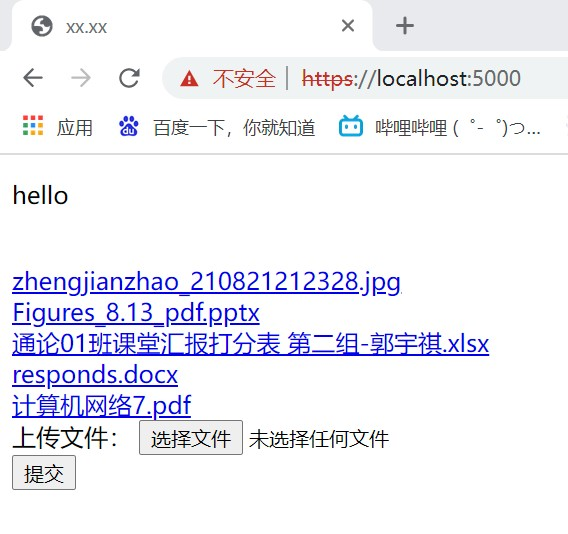
\includegraphics[width=0.4\textwidth]{figs/homepage.jpg}
  \caption{服务器主页示意图}
  \label{fig:homepage}
\end{figure}

因此服务器的文件上传下载功能运行良好。

\subsection{文件分块传输测试}

我们对文件下载操作实现了分块传输。在不使用分块传输时,浏览器下载文件状态如图\ref{nochunk}所示。由图可见,不使用分块传输时,客户端可以在文件下载完毕前通过Content-Length字段获得文件大小。
\begin{figure}[!h]
\begin{center}

\includegraphics[scale=0.8]{figs/nochunk.PNG}
\end{center}
\caption{不使用分块传输}
\label{nochunk}
\end{figure}

使用分块传输时,浏览器下载文件状态如图\ref{chunk}所示。由图可见,使用分块传输时,客户端在文件下载完毕前不能获取文件的总长度,只能得到已经下载的文件长度。

\begin{figure}[!h]
\begin{center}

\includegraphics[scale=0.8]{figs/chunk.PNG}
\end{center}
\caption{分块传输}
\label{chunk}
\end{figure}

\subsection{持久连接和管道测试}
为测试http管道,我们首先开启浏览器的管线化选项。为触发浏览器的管线化请求,我们实现了一个网页,路径为/img,用来展示上传文件中所有的图片。加载该网页须下载多个图片文件,支持管线化的浏览器会将这多个下载请求使用管线化技术发送。图\ref{pipeline}表明该网页能够正常加载所有图片,表明我们的服务端能良好支持管线化请求。

\begin{figure}[!h]
\begin{center}
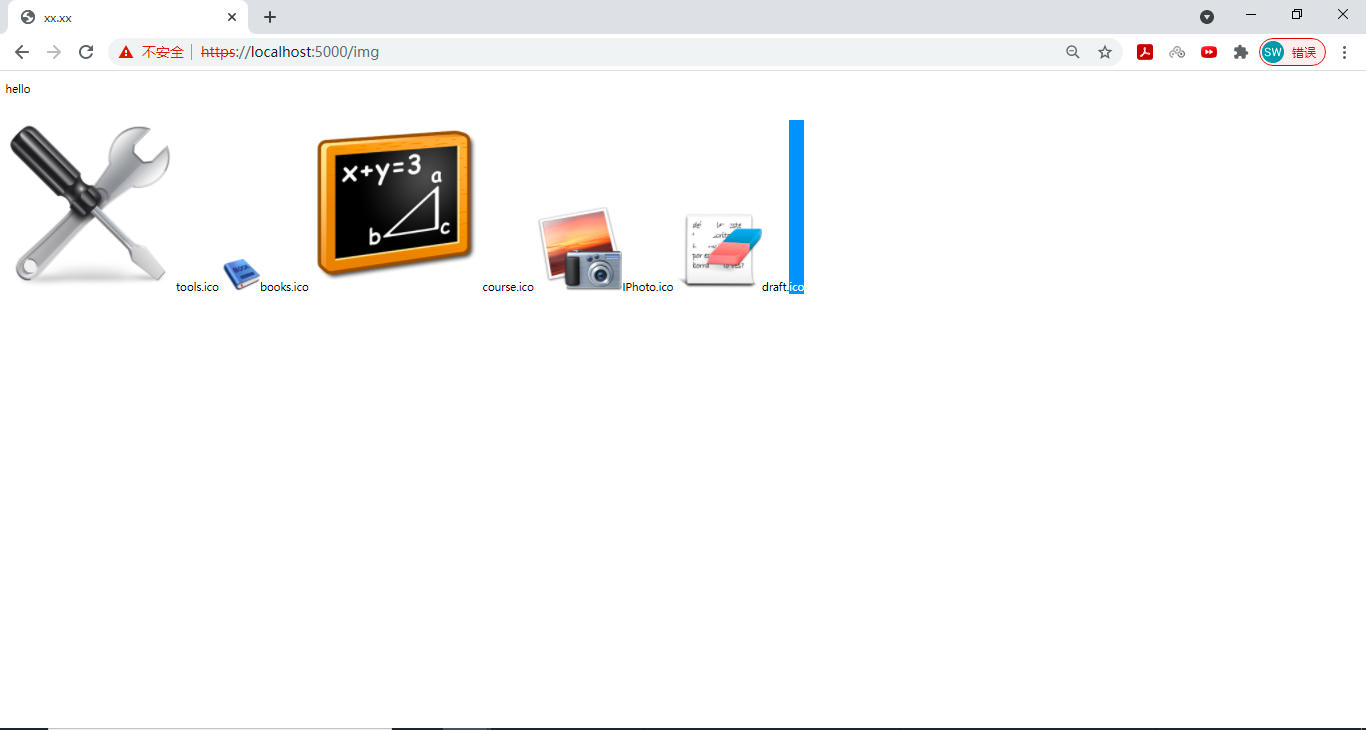
\includegraphics[width=0.7\textwidth]{figs/pipeline.PNG}
\end{center}
\caption{管线化}
\label{pipeline}
\end{figure}



\subsection{HTTPS测试}

我们使用openssl实现了https。这时访问服务器可以使用HTTPS协议。初次访问浏览器给出警告,如图\ref{warning}。这是因为我们自建的CA没有经过上层CA链的签名,无法验证服务器端身份。选择允许访问即可使用之前实现的功能。从浏览器端可以查看服务器证书,如图\ref{certificate},和对该证书进行签名的自建CA,如图\ref{ca}。
\begin{figure}
\begin{center}
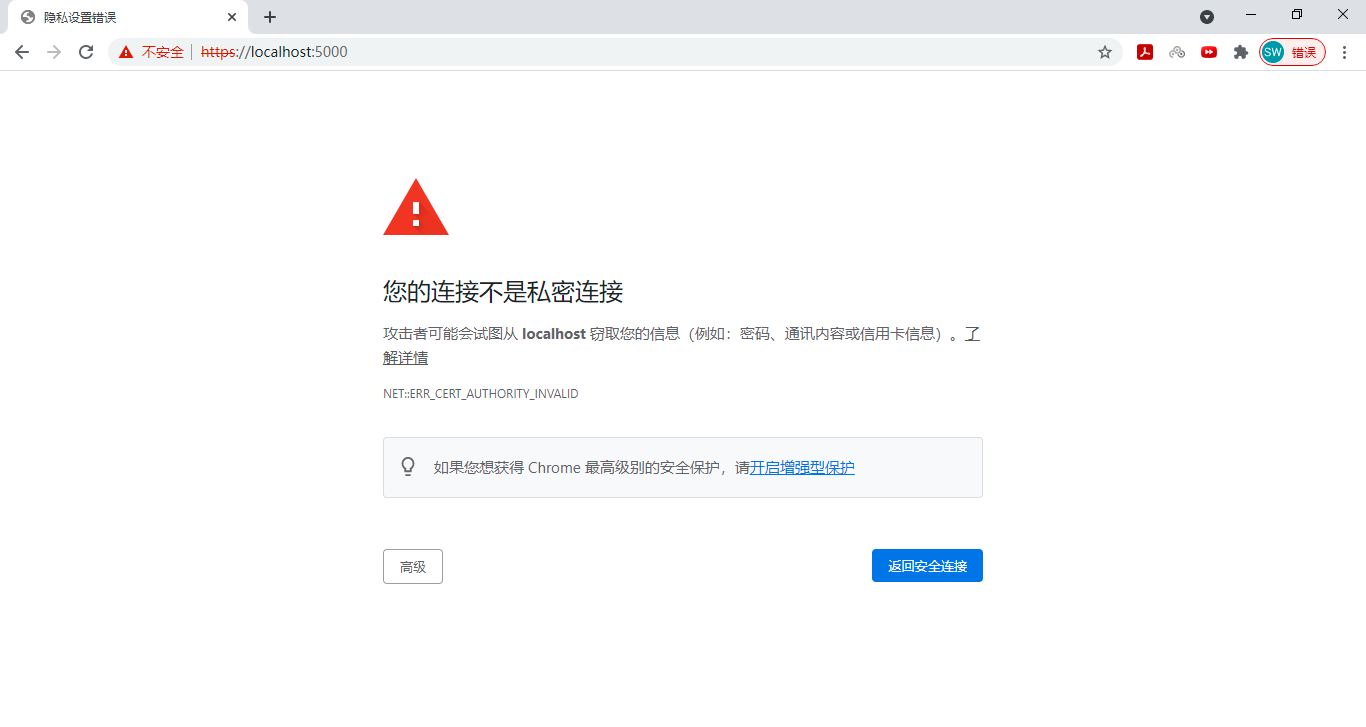
\includegraphics[width=0.8\textwidth]{figs/warning.PNG}
\end{center}
\caption{浏览器警告}
\label{warning}
\end{figure}

\begin{figure}
\begin{center}
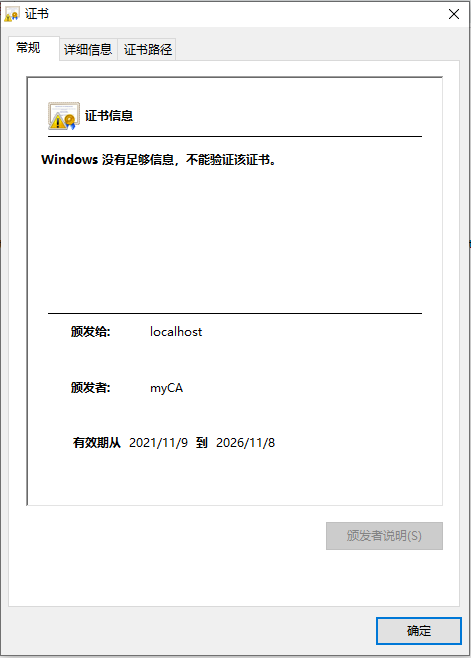
\includegraphics[scale=0.6]{figs/certificate.PNG}
\end{center}
\caption{证书}
\label{certificate}
\end{figure}

\begin{figure}
\begin{center}
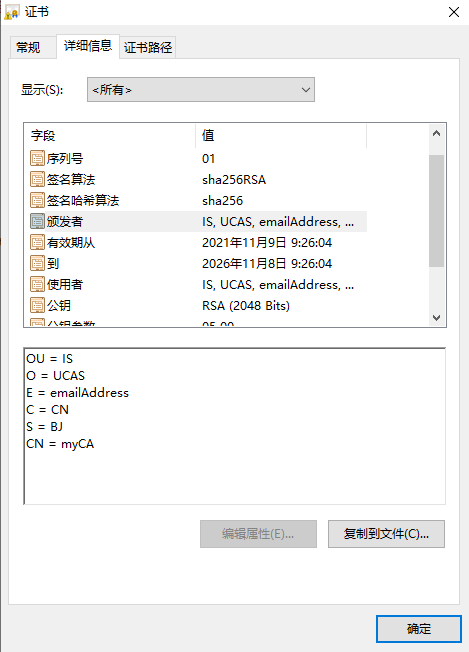
\includegraphics[scale=0.6]{figs/certificate2.PNG}
\end{center}
\caption{CA}
\label{ca}
\end{figure}

\subsection{多路并发测试}
我们在服务器上部署HTTP SERVER,并同时使用三台设备对服务器进行独立访问。在三台设备上,服务器均表现良好,返回内容均正常。因此服务器的多路并发功能完好。

\end{document}